\chapter{Introduction}

Clustering is an unsupervised machine learning method that groups similar observations together. Due to its ability to find patterns in an unlabeled dataset, its an essential task in Data Mining and Knowledge Discovery. A \textit{cluster} is a group of similar instances that belongs to a \textit{centroid} (center point of a cluster). Distance-based clustering algorithms use distance measures such as Euclidean distance to calculate the similarity of data points. Hierarchical methods partition the instances and merge (agglomerative) or split them into bigger or smaller clusters. Many other methods exist \cite{mixed_type_survey_2019}, but this work focuses on methods for clustering \textit{mixed-type} data.

\chapter{Related Work}

Lots of research has been put into creating deep neural network classifiers for the tabular data domain that try to beat Gradient boosted decision trees \cite{deep_neural_networks_tabular_data_survey}. There has been some research on incorporating attention or a Transformer block into such networks. TabNet \cite{tabnet} is a self-supervised classifier using attention that makes use of feature selection to group features into semantic categories. TabTransformer \cite{tab_transformer} and FT-Transformer \cite{ft_transformer} both use a full Transformer block before feeding the tensors into a MLP classifier. TabTransformer uses embeddings only for categorical features and uses a shared embedding to distinguish classes in one column from the classes in other columns. It then uses a Transformer block to attend the categorical features. FT-Transformer also uses embeddings for continuous features but no shared embedding. Using embeddings for both categorical and continuous features allows it to utilize all features in the Transformer block. There has also been research on classifiers that utilize attention not only over the features of one instance, but over multiple instances of a datasets \cite{attention_between_datapoints, saint}.

In the field of deep clustering, research of the last few years has focused on models that are able to learn clustering friendly representations, instead of sequentially connecting an autoencoder and a clustering module. DCN \cite{dcn} uses a joint loss function to update the autoencoder (representation module), the cluster assignments and centroids. DEC \cite{dec} has introduced a whole category of deep clustering methods, which minimize the Kullback-Leibler divergence between the cluster assignment distribution and an auxiliary distribution that is more centered around the cluster centroids. Some methods that fit in this category are: IDEC \cite{idec}, which improves DEC by including the reconstruction loss of the autoencoder; DEPICT \cite{depict}, which uses a convolutional autoencoder; DEC-DA \cite{dec-da}, which improves DEC by using data augmentation. Still, DCN and DEC provide the baseline for deep clustering in the image and natural language domain, which newer models are compared against.

\chapter{Foundation}

\section{Methodology}

\subsection{Datasets} \label{Datasets}

In this work we use 8 mixed-type datasets from the UC Irvine Machine Learning Repository \cite{uci_ml_rpo}.
The Abalone dataset \cite{abalone} contains physical measurements from abalones. It has 4177 instances, one categorical feature and seven continuous features.
The Auction Verification dataset \cite{auction_verification} has 2043 instances that contain verification runs of multi-round auctions. It is composed of six categorical and one continuous feature.
The Bank Marketing dataset \cite{bank_marketing} is related to a direct marketing campaign of a portuguese banking institution. It has 49732 instances, but was downsampled to 5000 random instances. The "age", "day" and "month" features were removed, which results in eight categorical and five continuous features.
The Breast Cancer dataset \cite{breast_cancer} contains 699 instances and 9 categorical features.
The Census Income dataset \cite{census_income} has a total of 48842 instances. It was downsampled to 5000 random instances. It is composed of eight categorical and 6 continuous features.
The Credit Approval dataset \cite{credit_approval} contains information of applications for credit cards. It has 690 instances, nine categorical features and six continuous features.
The Heart Disease dataset \cite{heart_disease} is composed of four datasets and has 920 instances in total. It has seven categorical features and six continuous features.
The Soybean (Large) Dataset \cite{abalone} consists of 683 instances from soybeans with a certain disease and has 35 categorical features.

All instances containing missing values were removed. Duplicate instances were explicitly not removed, since there is no information available if they are duplicates by accident, or real duplicates. Categorical features were standardized by removing the mean and scaling to unit variance, using the scikit-learn Python library \cite{scikit_learn}. Formally, the standardized score $z$ of a sample $x$ from a feature is calculated as
$$z = \frac{(x-\mu)}{\sigma},$$
where $\mu$ is the mean of the samples $x_1, ...,x_N$ from a feature of length $N$, defined as
$$\mu = \frac{1}{N} \sum^{N}_{i=1} x_i$$
and $\sigma$ is the standard deviation of the samples of a feature, defined as
$$\sigma = \sqrt{\frac{1}{N} \sum^{N}_{i=1}(x_i - \mu)^2}.$$
The datasets were shuffled. For all random operations, a random state of integer value 0 was used to ensure reproducibility. When using the PyTorch Python library \cite{pytorch} for implementing neural networks, a flag was set to only use deterministic algorithms.

\subsection{Evaluation} \label{Evaluation}

The clustering results were each evaluated with two measurements, \textit{Accuracy} and \textit{Normalized Mutual Information}. Accuracy is defined as 
$$\frac{\text{Instances predicted correctly}}{\text{Total number of instances}}.$$
Since any clustering algorithm will assign arbitrary class labels to each instance that might not align with the ground truth class labels, we map the predicted label classes to ground truth label classes in a way maximize the number of correctly predicted instances. This is an inversion of the \textit{Linear Assignment Problem}, we use an implementation provided by the Scipy Python library \cite{scipy} to solve this problem and find the optimal solution. 

As shown in Chapter \ref{Experiments}, some clustering methods falsely assign almost all instances to one target class. Because a part of the datasets we used are heavily imbalanced, this leads to unjustified high accuracy scores. Therefore, we use another metric, Normalized Mutual Information. It is based on \textit{Mutual Information}, which, for the ground truth labels $U$ and the predicted labels $V$ (switching both variables will not change the outcome) is defined as
$$\text{MI}(U,V) = \sum^{|U|}_{i=1}\sum^{|V|}_{j=1} \frac{|U_i \cap V_j|}{N} log\frac{N|U_i \cap V_j|}{|U_i||V_j|}$$
where $|U_i|$ is the number of instances assigned to cluster $U_i$ and $|V_i|$ is the number of instances assigned to cluster $V_i$ \cite{scikit_learn}. Normalized Mutual Information is Mutual Information normalized by the mean of the Entropies of $U$ and $Y$ \cite{scikit_learn}:
$$\text{NMI}(U,V) = \frac{\text{MI}(U,V)}{\frac{1}{2}(H(U)H(V))}.$$

\section{Classical Methods for clustering Mixed-Type data} \label{Classical Methods for clustering Mixed-Type data}

\subsection{k-means} \label{k-means}

The most well known distance-based clustering method is k-means \cite{kmeans}. The goal is defined as follows: Suppose we have a finite set of $n$ instances $S=\{p_1, p_2, ..., p_n\} \in \R^m$ for a dataset with $m$ features, the target of k-means is to find optimal centroids $B=\{b_1, b_2, ..., b_k\} \subseteq \R^m$ for a given $k (\leq n) \in \N$ that minimize the sum of the squared Euclidean distance of each point in $S$ to its nearest centroid. Formally
$$\sum_{i=1}^n  d(p_i, B)^2$$
has to be minimized, where $d$ is the Euclidean distance from a point $p_i \in S$ to the nearest centroid in $B$ \cite{kmeans_np_hard}:
$$d(p_i, B) = min_{1 \leq j \leq k} d(p_i, b_j).$$
The Euclidean distance between two points $p$ and $q$ in an $n$-dimensional Euclidean space is defined as 
$$d(p, q) = \Vert p - q \Vert = \sqrt{(p_1 - q_1)^2 + (p_2 - q_2)^2 + ... + (p_n - q_n)^2}.$$
Finding the optimal centroids is a NP-hard problem, even for $d=2$, as shown by Mahajan et al. \cite{kmeans_np_hard}. The most common algorithm used for the k-means problem is a iterative refinement technique proposed by Lloyd \cite{kmeans_lloyd}. It is defined as follows
\begin{enumerate} 
	\item Randomly set $k$ initial cluster centroids $b_1^{(1)}, ..., b_k^{(1)}$.
	\item Assign each observation $p_i$ to the nearest centroid using squared Euclidean distance. This splits our instances into $S$ into $k$ sets $\{S_1^{(t)}, ..., S_k^{(t)}\}$.
	\item Recalculate the optimal position of each centroid using the mean distance to each instance assigned to the centroid: 
$$b_i^{(t+1)} = \frac{1}{|S_i^{(t)}|} \sum_{p_j \in S_i^{(t)}} p_j.$$
	\item Repeat steps 2. and 3. until the centroid assignments no longer change.
\end{enumerate}

\subsection{k-modes} \label{k-modes}

In many real-world scenarios, besides continuous, numerical data, \textit{categorical} data exists. While Euclidean distance or other distance measures work well with continuous data, categorical data is different. Suppose we have categories $\{A, B, C\}$ of a given feature, we would encode them into numeric values to allow for computation of a distance measure:
$$\{A, B, C\} \equiv \{1, 2, 3\}.$$
While $A$ and $C$ can share the same semantic similarity as $A$ and $B$, numerically category $A$ and Category $C$ are now $|1-3| = 2$ apart, while Category $A$ and $B$ are only $|1-2|=1$ apart. During clustering, this could lead to instances being assigned to centroids based on a wrong distance assumption.

A possible solution is to use \textit{one-hot encoding}, also known as \textit{dummy coding} in classical statistics. One-hot encoding turns a discrete feature containing $k$ mutually exclusive categories into a vector $x$ of length $k$, in which only one of the elements $x_k$ equals 1 and all remaining elements equal 0 \cite{pattern_recognition_machine_learning}. For an instance $B$ of a feature having $k=3$ separate categories $\{A, B, C\}$, the one-hot vector $x$ would be represented by $x = (0, 1, 0)^{\intercal}$. According to Huang \cite{kmodes}, one-hot encoding has two drawbacks:
\begin{enumerate} 
	\item In real-world applications, categorical features with hundreds or thousands of categories are encountered. This would result in a large number of binary features in the one-hot encoded representation, which will increase cost and space of computation.
	\item The centroid value of a certain one-hot encoded feature, given by a real value between 0 and 1, cannot indicate the characteristics of the according cluster, since the feature only describes the presence or absence of one category.
\end{enumerate}
Therefore, Huang \cite{kmodes} proposed using the Kronecker-Delta as a dissimilarity measure between multiple categorical features. Formally, if we have two instances $X$ and $Y$ of a dataset with $m$ categorical features, $d_1$ will count the number of mismatches between the categorical features of both instances, defined as
$$d_1(X, Y) = \sum^m_{j=1} \delta (x_j, y_j)$$
where the Kronecker delta $\delta (x_j, y_j)$ is defined as
$$\delta (x_j, y_j) = 
\begin{cases}
    0 & (x_j = y_j)\\
    1 & (x_j \neq y_j)
\end{cases}.
$$
If we have a finite set of $n$ instances $S=\{p_1, p_2, ..., p_n\}$ for a dataset with $m$ categorical features, the goal of \textit{k-modes} \cite{kmodes} is to find optimal \textit{modes} $B=\{b_1, b_2, ..., b_k\}$ for a given $k (\leq n) \in \N$ that minimize
$$\sum_{i=1}^n  d_1(p_i, B)$$
where
$$d_1(p_i, B) = min_{1 \leq l \leq k} \sum^m_{j=1} \delta (p_{i,j}, b_{l,j}).$$
Similar to k-means, we can use an iterative algorithm for efficient computation \cite{kmodes}:
\begin{enumerate} 
	\item Randomly choose $k$ instances from the dataset as initial modes for the clusters.
	\item Assign each instance to their nearest mode using the proposed dissimilarity measure one by one and update the mode of each cluster after each assignment.
	\item Test if each instance still belongs to its assigned mode, i.e. if each instance is assigned to its nearest mode. If the instance would belong to a different mode, reassign the instance and update the modes of both clusters.
	\item Repeat step 3. until the mode assignments no longer change.
\end{enumerate}

\subsection{k-prototypes}

As proposed by Huang \cite{kmodes}, it is straightforward to combine the k-means and k-modes algorithms into the \textit{k-prototypes} algorithm, which can be used to cluster \textit{mixed-type} data (consisting of numerical, continuous and categorical features). The dissimilarity between two instances $X$ and $Y$ with features $A^r_1, A^r_2, ..., A^r_s, A_{s+1}^c, ..., A^c_m$, where features $A^r_1, ..., A^r_s$ are continuous and features $A_{s+1}^c, ..., A^c_m$ are categorical, is defined as
$$d_2(X,Y) = \sum^s_{j=1}(x_j - y_j)^2 + \gamma \sum^m_{j=s+1}\delta(x_j, y_j).$$
The first part of the equation is the Euclidean distance as used in k-means, while the second part is taken from the k-modes algorithm. Huang \cite{kmodes} states: "The weight $\gamma$ is used to avoid favouring either type of attribute".

Again, we need to find $k$ optimal centroids $B=\{b_1, b_2, ..., b_k\}$ and therefore have to minimize
$$\sum_{i=1}^n  d_2(p_i, B)$$
where
$$d_2(p_i, B) = min_{1 \leq l \leq k} \sum^s_{j=1}(p_{i,j} - b_{l,j})^2 + \gamma \sum^m_{j=s+1}\delta(p_{i,j}, b_{l,j}).$$
We can minimize both distance measures at the same time since they are nonnegative. Therefore, we can use the same algorithm as defined in \ref{k-modes}. \cite{kmodes}

\subsection{Gower distance}

\textit{Gower distance} \cite{gower} is a general similarity measurement between instances containing mixed-type features. It is defined as follows: When comparing instances $x_i$ and $x_j$, for each feature $k$ of $p$ total features, we calculate a score $s_{ijk} \in [0,1]$. The score will be close to 1 for two instances $x_{ik}$ and $x_{jk}$ of a feature $k$ if they are similar, and close to 0 they are not similar.
Gower distance is also computable between instances with missing values, therefore a quantity $\delta_{ijk}$ is calculated, which is equal to 1, when feature $k$ can be compared across the two instances $x_i$ and $x_j$, and 0 otherwise (illustrated in Figure \ref{gower_dichotomous}).
Gower distance then is the average of the known score
$$S_{ij} = \frac{\sum^p_{k=1}s_{ijk}\delta_{ijk}}{\sum^p_{k=1}\delta_{ijk}}.$$
The Score $s_{ijk}$ is calculated differently according to the type of feature \cite{gower}:
\begin{enumerate}
	\item For \textit{dichotomous} (when a value is either present or absent) features, the score $s_{ijk}$ is 1 when the value is present in both features and 0 otherwise, as shown in Figure \ref{gower_dichotomous}.
	\item For categorical features, the score $s_{ijk}$ is 1 if they both instances match on feature $k$ and 0 otherwise.
	\item For continuous features the score is calculated as
	$$s_{ijk} = 1-\frac{|x_i-x_j|}{R_k}$$
	where $R_k$ is the range of feature $k$ in the dataset or in the sample.
\end{enumerate}
\begin{figure}
\centering
	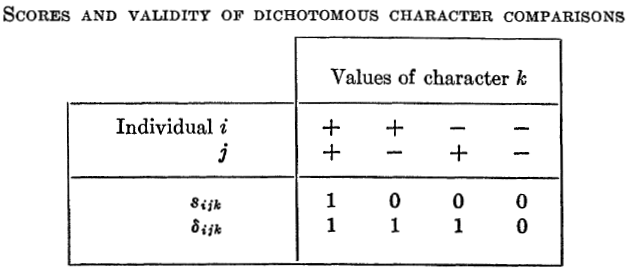
\includegraphics[width=\linewidth]{gower-dichotomous.png}
	\caption{Illustration from the original paper by Gower \cite{gower}. Score $s_{ijk}$ and quantity $\delta_{ijk}$ of a feature $k$ on two instances $x_i$ and $x_j$. Presence of a feature is denoted by "+" and absence by "-".}
	\label{gower_dichotomous}
\end{figure}
Gower \cite{gower} has shown that $\sqrt{1- S_{ij}}$ is a valid distance representation for two instances $x_i$ and $x_j$. We can now convert our similarity matrix $S$ into a distance matrix and are able to use Hierarchical clustering methods \cite{algorithms_for_clustering_data}. Philip and Ottaway \cite{philip_ottaway} used Gower distance with agglomerative clustering. Agglomerative clustering places each instance into its own cluster and recursively merges the clusters together using the given distance matrix, until only the specified number of clusters is remaining \cite{algorithms_for_clustering_data}.

\section{Deep Clustering}
\subsection{Neural Networks} \label{Neural Networks}

The idea of computation by neurons inspired by the human brain was first formalized into a mathematical model by McCulloch \cite{neural_network_1943}. A \textit{neuron} was defined as a element that takes multiple boolean inputs and has one boolean output. The neuron \textit{fires}, meaning the output is set to true, when the sum of the input values extends a certain threshold.

The single-layer \textit{perceptron}, the first neural machine learning algorithm, was invented by Rosenblatt in 1957 \cite{perceptron}. Formally, the binary valued output $o_j$ given an input vector $x_i$ is calculated as
$$o_j = 
\begin{cases}
    1 & \sum_i w_{ij}x_i + b > 0\\
    0 & otherwise
\end{cases}
$$
where $w$ is the learnable weight matrix, and $b$ is a predefined bias. For training, the weights $w$ are simply incremented when the output is 0 but the ground truth is 1, and decremented if the output is 1 but should be 0. If the output was predicted right, no weights are changed.

The idea of neural networks was revived three decades later, using multiple perceptron layers and a differentiable error function \cite{hidden_layer_backprop}. In a multi-layer neural network, we have an input layer, an output layer and multiple hidden layers. Each layer is a collection of neurons, that acquire the outputs of each neuron from the previous layer (or from the input in case of the input layer) as their input, and produce a new output. Formally, the output $a_j$ of the $j$th neuron of layer $n$ that gets $d$ input values from the previous layer is defined as
$$a_j = \sum^d_{i=1}w_{ji}^{(n)}x_i + b_j^{(n)}$$
where $w_{ji}^{(n)}$ is the learnable weight of the input $x_i$ going through neuron $j$ in layer $n$ \cite{neural_networks_pattern_recognition}. A bias $b_j$ is also added. This output is commonly referred to as an \textit{activation} of a neuron \cite{neural_networks_pattern_recognition}. Because every neuron is a linear function, in order to avoid the collapse of each neuron from all layers into a single linear function, we pass the activation $a_j$ into a non-linear activation function $f$
$$z_j = f(a_j)$$
before being passed to the next layer of neurons \cite{activation_functions}.

\begin{figure}
\centering
	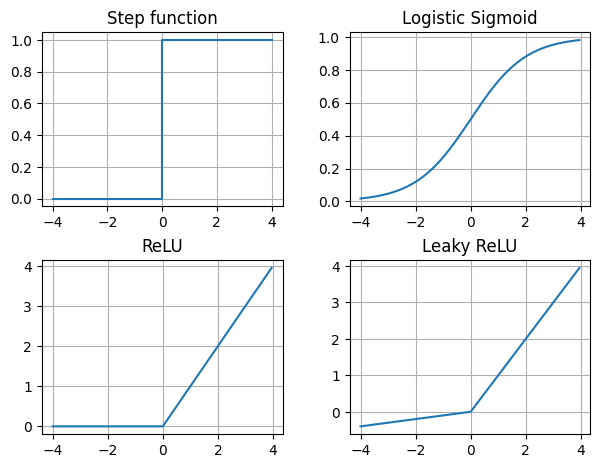
\includegraphics[width=0.8\linewidth]{activation-functions.png}
	\caption{An illustration of the step function, the logistic sigmoid, the ReLU and the Leaky ReLU activation functions.}
	\label{activation_functions}
\end{figure}

As shown in a recent survey \cite{activation_functions}, there are many different activation functions used in neural networks. A simple example for an activation function, which naturally aligns with the idea of a biological neuron firing is the \textit{step function} (also known as \textit{Heaviside step function}) \cite{neural_networks_pattern_recognition}, that outputs 0 for negative values and 1 for positive values:
$$\text{step function}(x) = 
\begin{cases}
    1 & x \geq 0\\
    0 & x < 0
\end{cases}.
$$
In order to stay between 0 and 1, but also utilize all real values in between, another activation function that has historically been popular is the \textit{logistic sigmoid} function \cite{activation_functions}, that squashes any input in $]0, 1[$:
$$\text{logistic sigmoid}(x) = \frac{1}{1 + e^{-x}}.$$
Because the outputs are in a range close to 0, it is prone to the \textit{vanishing gradient problem}. In the vanishing gradient problem, a gradient that is very close to 0 leads to almost no update in the weights of the network during training. Moreover, using a exponential value naturally leads to a greater computational complexity. \cite{activation_functions}

The current state-of-the-art activation function, the \textit{Rectified Linear Unit} (ReLU) \cite{activation_functions}, is not limited by the above disadvantages. It is simple and computationally performant. It is defined as the identity for positive values and as 0 for negative values:
$$\text{ReLU}(x) = max(0, x) = 
\begin{cases}
    x & x \geq 0\\
    0 & x < 0
\end{cases}.
$$
One downside of the ReLU activation function is that there will be a substantial amount of dead neurons in the network (neurons with output 0 will not affect the neurons of the next layer). The \textit{Leaky Rectified Linear Unit} (Leaky ReLU or LReLU) \cite{activation_functions} utilizes negative values as well, but with a small coefficient, usually set to $0.01$. It is defined as
$$\text{Leaky ReLU}(x) = 
\begin{cases}
    x & x \geq 0\\
    0.01 \times x & x < 0
\end{cases}.
$$
All four activation functions are illustrated in Figure \ref{activation_functions}.

In a multi layer neural network, we need to be able to update the weights during training, so the network can learn the most optimal weights in order to fulfill its designated task. In the single layer perceptron, we were able to change the weights directly based on the predicted output, but in a multi layer network this is non-trivial, since we have multiple such perceptron layers that are sequentially attached. The solution is to use differentiable activation functions (or activation functions differentiable at almost every point, e.g. ReLU is not differentiable at 0), so each neuron together with its activation function becomes a differential function of the input, the weight and bias. We can now define a differentiable error function of the network outputs, which therefore is also a differentiable function of the weights. A common error function used in neural networks is the \textit{mean squared error}, defined as
$$\text{MSE} = \frac{1}{n} \sum^n_{i=1}{(y_i - z_i)^2},$$
where $n$ is the number of input instances, $y_i$ ist the target label of instance $x_i$ and $z_i$ is the network output on instance $x_i$. The derivatives of the error function in combination with stochastic gradient descent can be then be used to find the weights that minimize the error function. \cite{neural_networks_pattern_recognition}

\subsection{Autoencoder}

A neural network, as defined in the previous section, needs the target labels of a dataset in order be trainable. In a unsupervised learning setting, this is unapplicable. An approach used for pre-training neural networks with unlabeled data is using an \textit{autoencoder} neural network, first formalized by Ballard \cite{autoencoder}. An autoencoder is a neural network, that projects the input into a lower-dimensional embedding space, and then back into its original dimensionality. The network tries to reconstruct the original input the best it can, after it was encoded into the embedding space. Therefore the target label fed into the loss function is the original input. This allows such a network to be trained without the need for labeled data. The autoencoder consists of two blocks, where each is a collection of fully connected linear layers. The \textit{encoder} maps the input into the embedding space, while the \textit{decoder} projects the encoded representation into its original dimensionality. Both blocks can contain multiple hidden layers, but typically they are constructed symmetrical, meaning the number and size of the linear layers in the decoder are the same as in the encoder, but inverted (illustrated in Figure \ref{autoencoder_illustration}). 

\begin{figure}
\centering
	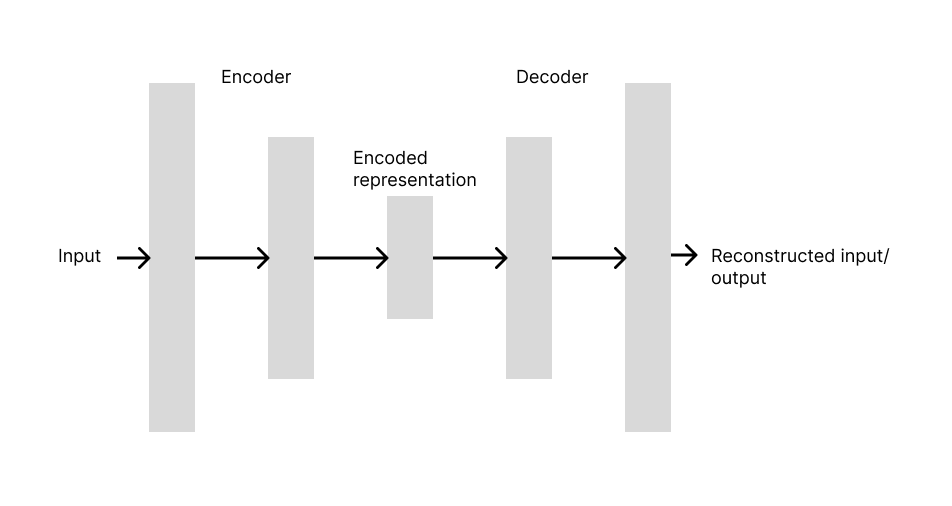
\includegraphics[width=1.1\linewidth]{autoencoder.png}
	\caption{Illustration of an autoencoder neural network.}
	\label{autoencoder_illustration}
\end{figure}

In unsupervised learning such as clustering, the autoencoder can be used to learn a dense representation of the input data. After training, we can feed the data into the encoder part of the autoencoder in order to obtain the encoded data, before utilizing a classical clustering algorithm to acquire the final cluster labels. The encoded representation has a smaller dimensionality and only contains the most relevant parts of the data (which were needed for reconstruction), which can benefit clustering.

\subsection{Deep Clustering} \label{Deep Clustering}

The problem of training an autoencoder before clustering is that the autoencoder cannot learn a suitable representation for the subsequent clustering step. The autoencoder has no objective that rewards learning a cluster-friendly representation \cite{dcn}. Instead of using a multi-stage process that splits autoencoder training and clustering, recent research has focused on a variety of of solutions that combine feature representation learning and clustering \cite{deep_clustering_survey}. The general goal is to learn feature representations that are suitable for clustering.

\begin{figure}
\centering
	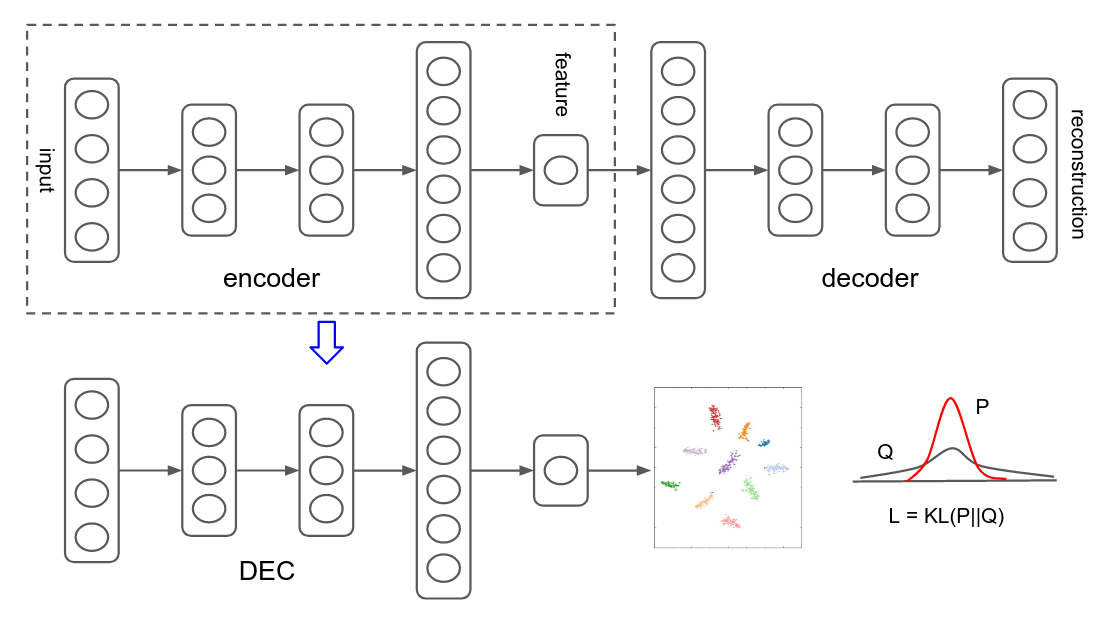
\includegraphics[width=1\linewidth]{dec.png}
	\caption{Illustration of DEC by Xie et al. \cite{dec}.}
	\label{dec}
\end{figure}

\begin{figure}
\centering
	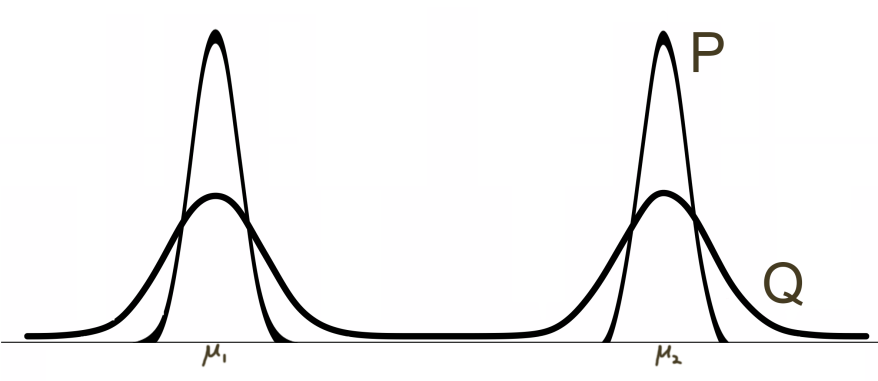
\includegraphics[width=0.7\linewidth]{p-and-q-distributions.png}
	\caption{Illustration from Li \cite{comparing_DEC_and_DCN} on the distributions $Q$ and $P$ on two cluster centroids $\mu_1$ and $\mu_2$. It is notable that $P$ is more concentrated around the cluster centers, but still derived from $Q$.}
	\label{p-and-q-distributions}
\end{figure}	

Xie et al. \cite{dec} proposed DEC (Deep Embedded Clustering), an approach using a iterative process that simultaneously learns feature representations and cluster assignments. DEC initially trains the autoencoder on the data as with the previous multi-stage approach, but then leaves out the decoder, as illustrated in Figure \ref{dec}, and trains the encoder separately while clustering to learn more optimal feature representations. After the initial autoencoder pre-training, standard k-means (Section \ref{k-means}) is used on the encoded representation to obtain initial cluster labels. A two-step algorithm is then used to iteratively update both the cluster assignments and feature representations. The first step involves computing a \textit{soft assignment} between the encoded data points and the cluster centroids. Student's $t$-distribution is used as a kernel, with fixed degrees of freedom $\alpha = 1$:
$$q_{ij} = \frac{(1 + \Vert z_i - \mu_j \Vert^2 / \alpha)^{-\frac{\alpha+1}{2}}}{\sum_{j'}(1 + \Vert z_i - \mu_{j'} \Vert^2 / \alpha)^{-\frac{\alpha+1}{2}}},$$
where $z_i$ represents the encoded value of instance $x_i$ and $\mu_j$ the centroid value of cluster $j$. The resulting value $q_{ij}$ can be interpreted as the probability of assigning instance $x_i$ to cluster $j$. The objective of the second step is minimizing the Kullback-Leibler divergence between our previously defined distribution $Q$ and an auxiliary distribution $P$:
$$L = \text{KL}(P \Vert Q) = \sum_i \sum_j p_{ij} log\frac{p_{ij}}{q_{ij}}.$$
The auxiliary distribution $P$ is more concentrated around the cluster centers than $Q$ (illustrated in Figure \ref{p-and-q-distributions}), but not using an unnatural distribution such as a delta distribution. The goal of $P$ is to strengthen clustering predictions, put more emphasis on points assigned with high confidence and normalize loss contribution of each centroid. Therefore, $P$ is defined as
$$p_{ij} = \frac{q_{ij}^2 / f_j}{\sum_{j'}q_{ij}^2 / f_{j'}},$$
where $f_j = \sum_i q_{ij}$ is the soft cluster frequency. We can then train the encoder using stochastic gradient descent to produce points $z_i$ that minimize the Kullback-Leibler divergence. \cite{dec}

\begin{figure}
\centering
	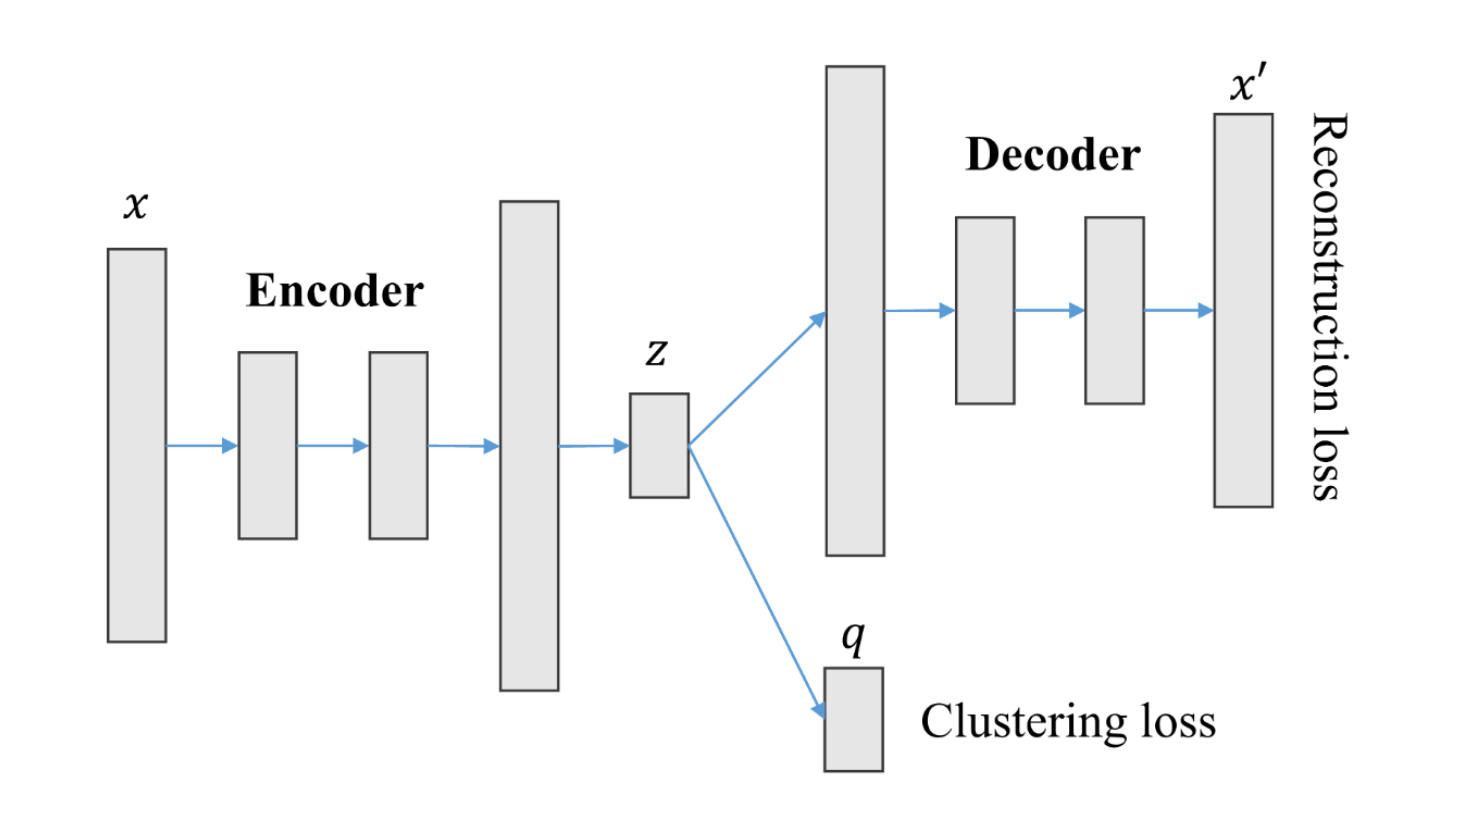
\includegraphics[width=0.7\linewidth]{idec.png}
	\caption{Illustration of IDEC by Guo et al. \cite{idec}.}
	\label{idec}
\end{figure}

Guo et al. \cite{idec} proposed IDEC (Improved Deep Embedded Clustering), which tries to improve DEC by also using the autoencoder reconstruction loss. Formally, the autoencoder reconstruction loss $L_r$ is added to the DEC loss $L_c = \text{KL}(P \Vert Q)$, which gives:
$$L = L_r + \gamma L_c,$$
where $\gamma > 0$ is a hyperparameter. This is illustrated in \ref{idec}.

\begin{figure}
\centering
	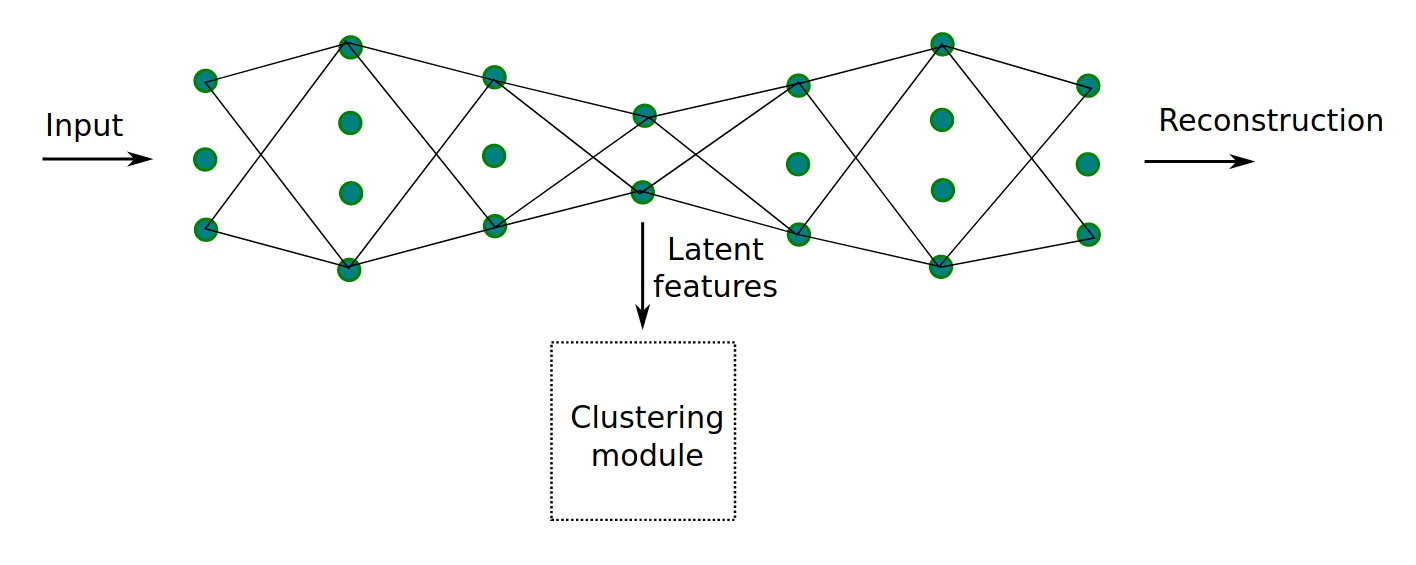
\includegraphics[width=0.9\linewidth]{dcn.png}
	\caption{Illustration of DCN by Yang et al. \cite{dcn}.}
	\label{dcn}
\end{figure}

Yang et al. \cite{dcn} proposed DCN (Deep Clustering Network) (Figure \ref{dcn}), which uses a joint loss function to optimize both feature representations and clustering predictions. The loss function is defined as
$$L = \sum^N_{i=1} \Big(\ell(g(f(x_i)), x_i)+ \frac{\lambda}{2}\Vert f(x_i)-Ms_i\Vert^2_2\Big).$$
The loss function consists of two parts, the reconstruction loss (first term of the sum) and the clustering loss (second term of the sum). $\lambda$ is used as a hyperparameter to balance the two terms. The network then alternates between updating the network parameters, updating the assignments to the cluster centroids and updating the cluster centroids themselves.

\chapter{Attention in Mixed-Type Clustering}

\section{Autoencoder and k-means} \label{Autoencoder and k-means}

It is difficult to formulate statistical distance measures for comparing two values of a categorical feature. Categorical features are irregular in nature, they can be binary, ordinal, non-ordinal or composed of many semantically different classes. This makes it hard to cluster a mixed-type datasets with classical clustering methods. As described by Huang \cite{kmodes} and also explained in Section \ref{k-modes}, one-hot encoding is suboptimal for the use in clustering tasks. The proposed solution by Huang, k-prototypes \cite{kmodes}, does not beat k-means or k-means with one-hot encoding on any tested dataset, as shown in Chapter \ref{Experiments}. Gower distance shows great accuracy results on all datasets and manages to beat the other methods on five out of eight datasets. As further illustrated in Chapter \ref{Experiments}, the accuracy evaluation metric is highly problematic, since some datasets are heavily imbalanced. In fact, the datasets on which gower distance achieves the best accuracy results are greatly imbalanced. This means the agglomerative clustering used with gower distance falsely assigns almost all instances to one target class. When looking at Normalized Mutual Information (NMI), gower distance with agglomerative clustering does not beat k-means or k-means with one-hot encoding on any dataset. This leaves us with naive k-means intended for only numerical, continuous data and k-means with one-hot encoding, which is a inefficient, suboptimal encoding.

Therefore, instead of using statistical distance measure to compare instances with categorical and continuous features, we use an autoencoder neural network to learn a dense representation of the data. The clustering architecture we build upon is a multi-stage process. We first train the autoencoder on our dataset independently of the clustering process. The training step is repeating many times, in our experiments we train the network a hundred times (hundred epochs). After the initial training step, we can feed the dataset into the encoder part of our trained autoencoder to get the dense, encoded representation of our data. We can perform k-means clustering over this representation to get the final cluster labels.

\section{Column Embeddings} \label{Column Embeddings}

Even when using neural networks, there is still the problem of representing categorical values, especially non-ordinal values, as explained in depth in Section \ref{k-modes}. Therefore, we use a learnable \textit{embedding} layer for categorical values. The resulting embedded tensor of the embedding layer for a categorical feature is a meaningful representation that is more dense that a one-hot encoded feature. The embedding layer is composed of a weight tensor $e_i$ for each categorical feature $i$. The weight tensor $e_i$  has the following dimensionality: $|i| \times s_i$, where $|i|$ is the number of unique classes in categorical feature $i$ and $s_i$ is the corresponding embedding dimension. We calculate the embedding dimension $s_i$ of feature $i$ as
$$s_i = min(50, \lceil \frac{|i|}{2} \rceil).$$
We then encode the classes of each categorical feature with integer values, going from 0 onwards. These integer values serve as indices for the corresponding weight tensor of our embedding layer. Passing a value $j$ of a feature $i$ in the embedding layer returns the one-dimensional tensor at index $j$ of the weight tensor $e_j$, which is of dimension $1 \times s_i$. The resulting tensors of each categorical feature from the embedding layer are concatenated into a tensor of size $1 \times \sum^n_{i=1}s_i$, where $n$ is the number of categorical features. To construct the complete input tensor, we concatenate the tensor of the embedded categorical features with the tensor of the continuous features. The continuous features of an instance are not embedded, but scaled by removing the mean and scaling to unit variance as explained in Section \ref{Datasets}. Having $m$ continuous features would result in a tensor of continuous features with size $1 \times m$. After concatenating both tensors, this leaves us with an input tensor of size $1 \times (m + \sum^n_{i=1}s_i)$. This input tensor can then be passed into the first linear layer of the encoder.

The goal of the autoencoder therefore is to reconstruct the embeddings, not the actual input. To be able to use a loss function on this network, we clone the tensor of the embedded categorical features and save it in a variable, and later compare the decoder output with the cloned embedded tensor (concatenated with the continuous features).

\section{Attention} \label{Attention}

\begin{figure}
\centering
	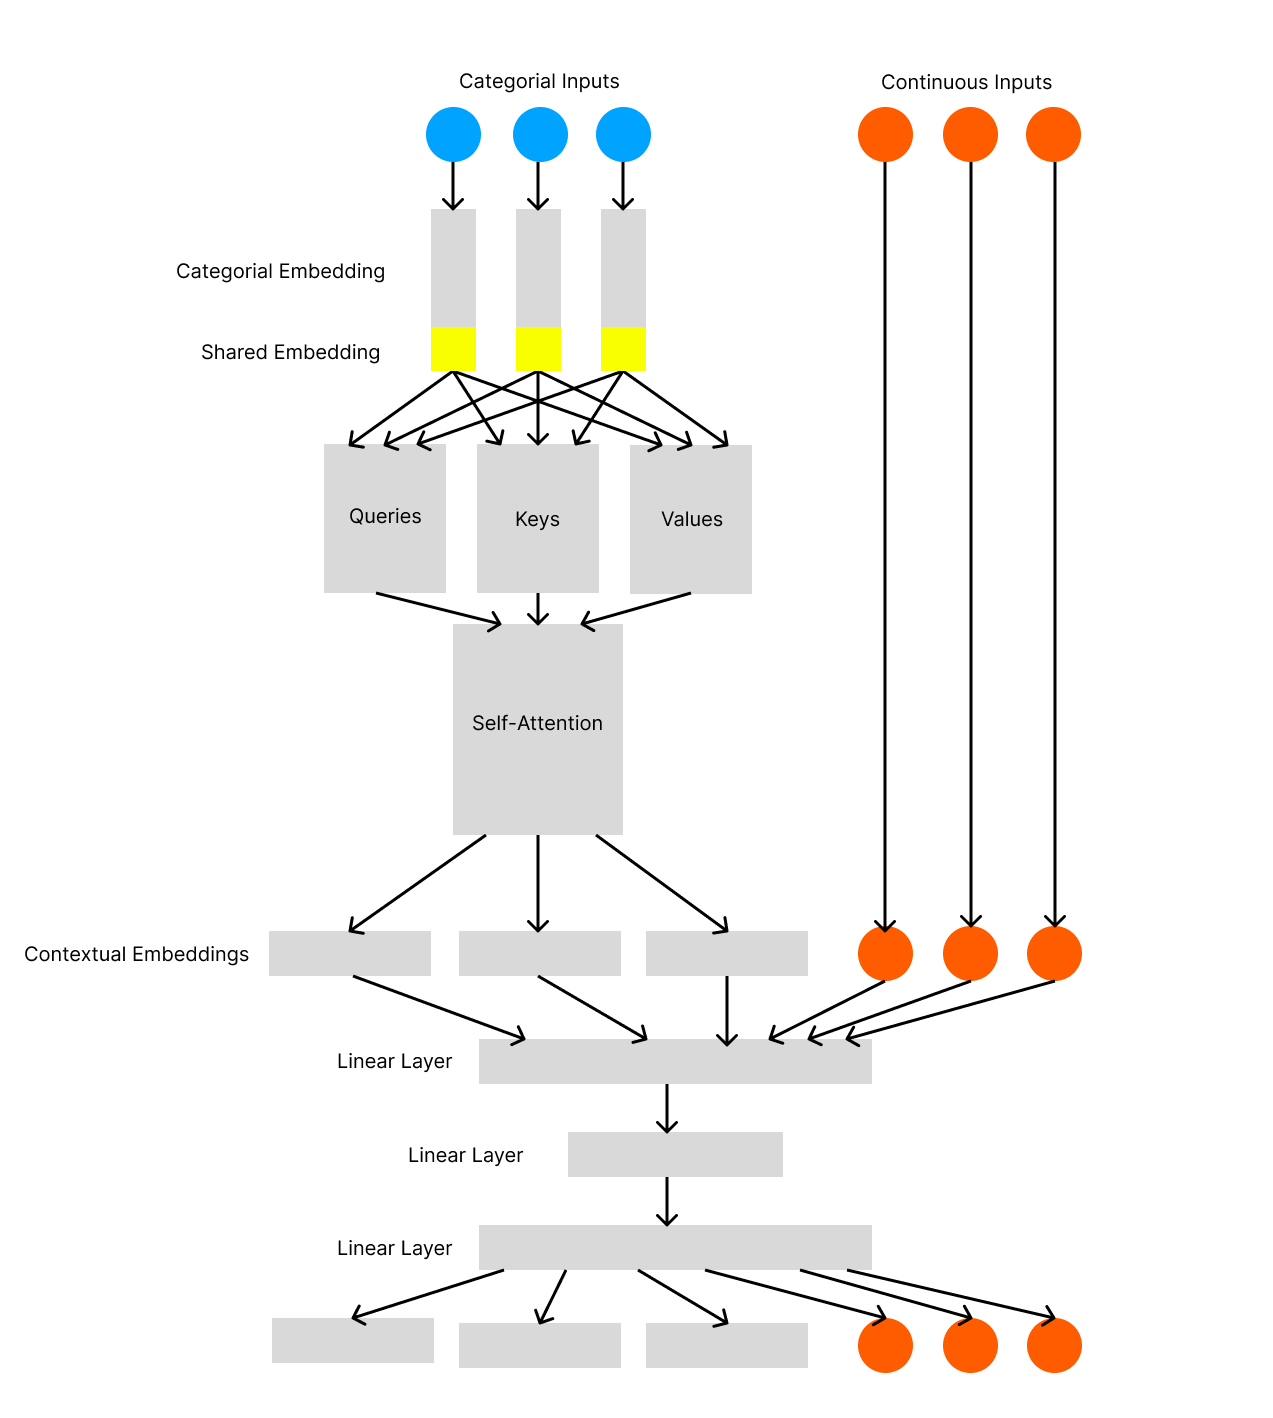
\includegraphics[width=1.2\linewidth]{attention_autoencoder.png}
	\caption{Architecture of the self-attention autoencoder network.}
	\label{attention_architecture}
\end{figure}

\textit{Self-attention} is a machine learning mechanism for sequence processing, originally used in machine translation by Bahdanau et al. \cite{bahdanau} and extended into the \textit{Transformer} architecture by Vaswani et al. \cite{attention_is_all_you_need}. It is a sequence-to-sequence operation, that aims to create a better representation of the input sequence by putting each element into the context of the other elements (paying "attention" to each other element). We do not operate with a sequence, but instead with multiple categorical features that might be related. For example, the relevance of a feature for the clustering process might depend of the value of another feature. The goal of the attention mechanism is to augment this feature (increase or decrease its vector representation) only when the other feature has this certain value. 

Self-attention operates with three input tensors: \textit{queries}, \textit{keys} and \textit{values}. Each of them is the input tensor, but used for different parts of the attention process. We add three independent linear projection to the input tensor to learn different representations for queries, keys and values. We apply attention to the categorical features after they were embedded in the embedding layer and then projected into queries, keys and values. The resulting vectors for each categorical feature are called \textit{contextual embeddings}, since they contain information on the context of the input sample. We concatenate these embedding vectors lengthwise, before passing them into the first linear layer of the encoder, as illustrated in Figure \ref{attention_architecture}.

\begin{figure}
\centering
	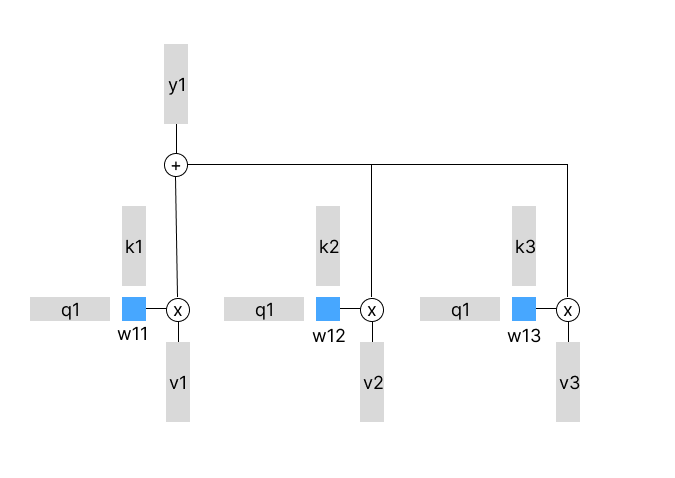
\includegraphics[width=1.1\linewidth]{attention_illustrated.png}
	\caption{Illustration of the attention mechanism on calculating the first output vector, inspired by Bloem \cite{transformers_from_scratch}. q1, k1, v1 represent the vectors at index 1 of Queries $Q$, Keys $K$ and Values $V$ respectively. The softmax function over the weights is not part of this illustration.}
	\label{attention_illustrated}
\end{figure}

Queries, keys and values are a sequence of $n$ vectors that have $d$ dimensions, resulting in dimensionality $n \times d$. In our case, the input dimension and therefore also the queries $Q$, keys $K$ and values $V$ are one-dimensional vectors, since the embedded vectors of each categorical features are concatenated along the first axis, as further illustrated in the previous section. We therefore cannot use our previously created input tensor. Because we calculate an individual embedding dimension (with a formula defined in the previous section) for each categorical feature, we cannot concatenate the vectors row-wise, since they all differ in length. Instead, we have to use a fixed embedding dimension $d$ for every categorical feature. Then, we can create tensors $Q$, $K$ and $V$ with dimension $n \times d$ each, where $n$ is the number of categorical features. The value 32 was chosen for embedding dimension $d$.

Because Attention is a mechanism that calculates values that combine multiple features, we need to be able to differentiate between the classes of different features, since we have a separate learnable embedding for each feature. A solution in the domain of text translation proposed by Vaswani et al. \cite{attention_is_all_you_need} is to add a positional encoding to each embedding in order to indicate the position of the word in the sentence. This is not suitable for tabular data, since the features do not have a particular order. We instead use a solution proposed by Huang et al. \cite{tab_transformer}, which uses a shared embedding across all categorical features. The goal of the shared embedding is to learn dissimilar representations for different classes of separate features in order to distinguish them. The shared embedding is a learnable tensor of size $n \times \frac{d}{8}$, that is concatenated to our input tensor in the first dimension. The fixed embedding dimension $d$ is therefore subtracted by 8, which results in a input tensor of categorical features of size $n \times d$. 

The first step of self-attention is to calculate attention weights for every element of the input sequence. For that, we will multiply every query of our queries with the keys. Formally, we can define this as a matrix multiplication:
$$W = QK^\intercal,$$
where $W$ are the resulting attention weights, $Q$ are the queries and $K$ the keys. The goal of this operation is to calculate weights $W_{ij}$ that indicate how important feature $i$ is to feature $j$ and vice versa. Each weight is an arbitrary value, therefore we use the softmax function \cite{neural_networks_pattern_recognition} to flatten the weights. The softmax function on a weight $w_{ij}$ is defined as
$$\text{softmax}(w_{ij}) = \frac{\exp(w_{ij})}{\sum_j{w_{ij}}}.$$
Because the weights $W$ can grow towards positive and negative infinity, in order to minimize the vanishing gradient problem of the softmax function (further explained in Section \ref{Neural Networks} in the case of the sigmoid function), we scale the attention weights by $\sqrt{d}$ before passing them into the softmax function:
$$W = \frac{QK^\intercal}{\sqrt{d}}.$$
We are scaling by $\sqrt{d}$, since its the average increase in Euclidean length of a weight vector $w$ when increasing its dimension $d$. \cite{attention_is_all_you_need}

Now after we have obtained the attention weights that indicate how important a feature is to every other feature, we need to multiply these weights with each feature vector. This will result in vectors that carry information to which other feature vectors we need to pay attention to. We use the remaining linear projected tensor, the values $V$, for this step. The full Attention mechanism is therefore defined as
$$\text{Attention}(Q, K, V) = \text{softmax}(\frac{QK^\intercal}{\sqrt{d}})V.$$
An illustration on how the first output vector in the attention mechanism is calculated is given by Figure \ref{attention_illustrated}.

\section{Transformer}

\begin{figure}
\centering
	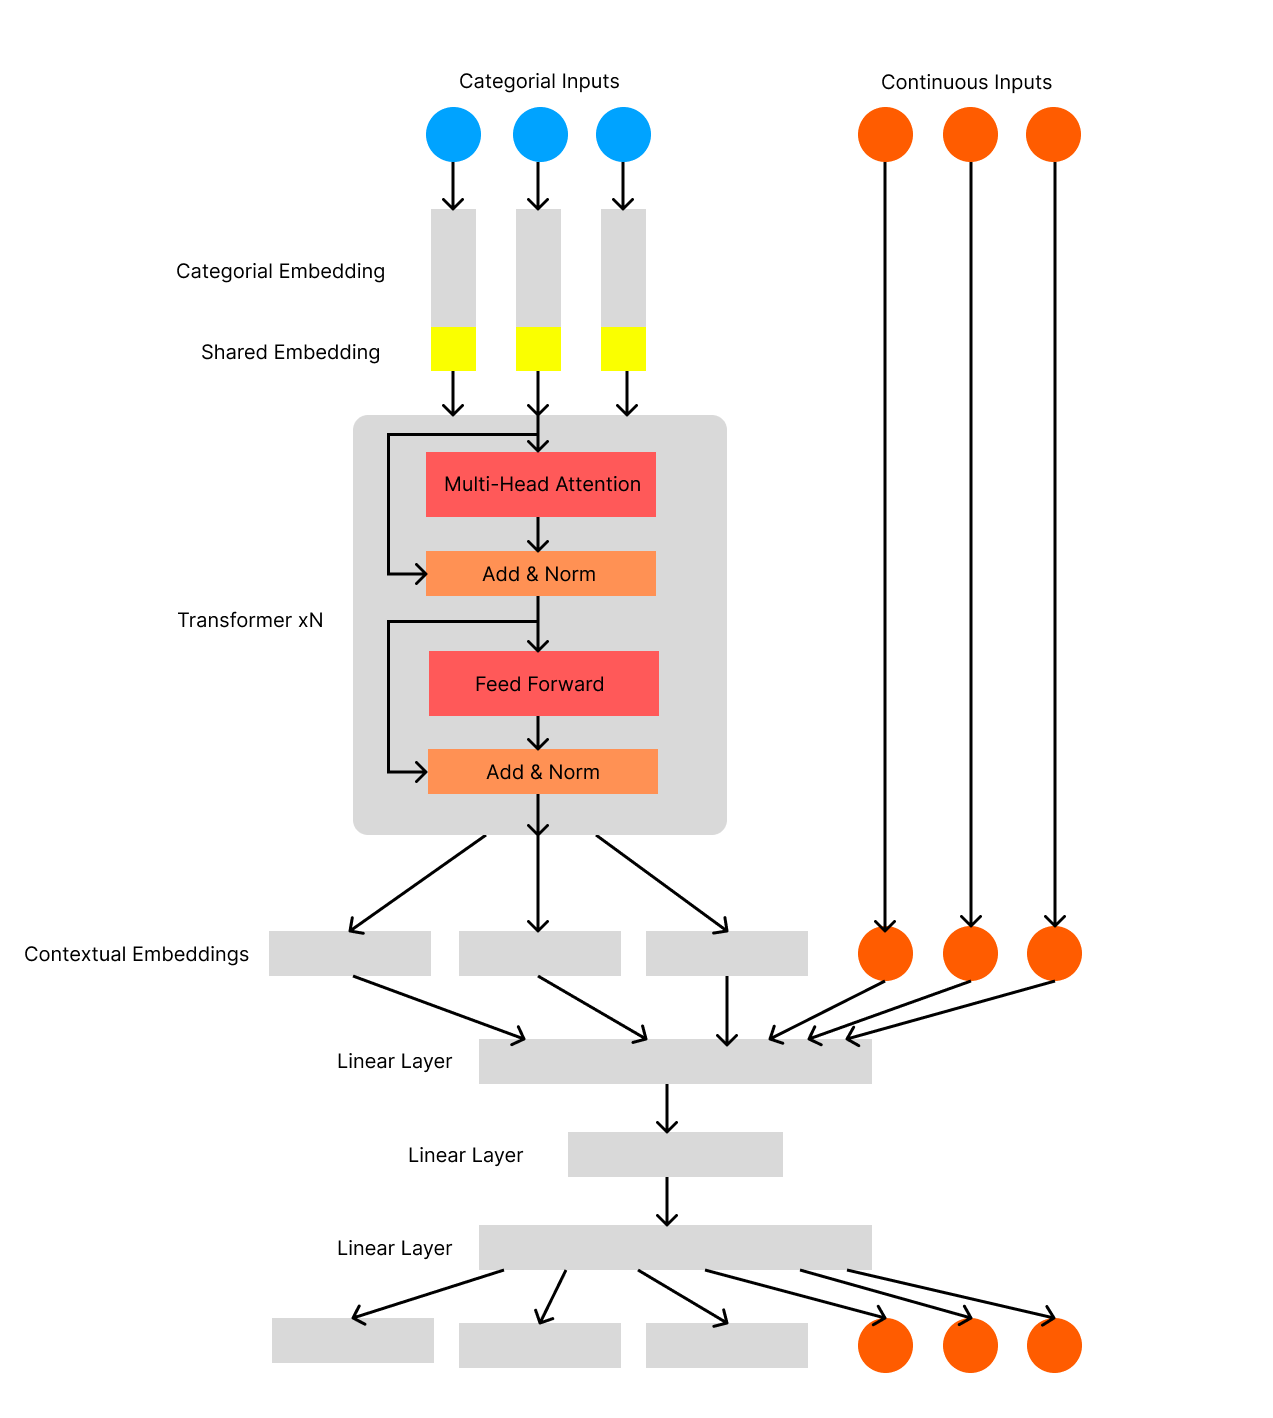
\includegraphics[width=1.2\linewidth]{transformer_autoencoder.png}
	\caption{Architecture of the Transformer autoencoder network.}
	\label{transformer_autoencoder}
\end{figure}

The \textit{Transformer} is a architecture based on the attention mechanism, first formalized by Vaswani et al. \cite{attention_is_all_you_need}. The Transformer extends attention into \textit{multi-head attention} and combines it with a feed-forward network and layer normalization. Multi-head attention \cite{attention_is_all_you_need} splits the input in $h$ parts and learns $h$ different representations for queries $Q$, keys $K$ and values $V$ respectively. Attention is then performed $h$ times in parallel using the different representations of $Q$, $K$ and $V$. This allows the model to perform attention over different subspaces of the embedded features at the same time. Using normal attention, we would only be able to attend to the complete embedding of the other features.

After performing attention, the Transformer adds the attention outputs to the initial input and normalizes this sum using \textit{layer normalization} \cite{layer_normalization}. The output is then fed into two linear layers, the first layer projecting the input to four times its size, and the second layer projecting it onto the original size again. Once again, the output is added to the input of the linear layers, and normalized using layer normalization. This process, illustrated in Figure \ref{transformer_autoencoder}, is sequentially applied $N$ times. The layer normalization and feed-forward network between each multi-head attention operation allow the model to parameterize the attention outputs. This makes sure the model can learn from each attention step.

The Transformer was originally designed for natural language tasks, but Huang et al. \cite{tab_transformer} proposed the \textit{Tab Transformer}, a multi-layer perceptron classifier for the tabular domain, based on the Transformer architecture. Inspired by the performance increase on mixed-type datasets using this architecture, we build a Transformer-based autoencoder network for clustering. The architecture, illustrated in Figure \ref{transformer_autoencoder}, is similar to the previous attention-based autoencoder but uses $N = 6$ Transformer blocks instead of one single self-attention block. Our categorical feature embedding size is 32 as previously. We perform multi-head attention with $h = 8$ heads, yielding a embedding dimension for each head of $\frac{d}{h} = 4$.

\subsection{FT-Transformer}

Gorishniy et al. extends the Tab Transformer into the \textit{FT-Transformer}, which uses embeddings for the numerical features as well. We implement a FT-Transformer autoencoder network, illustrated in Figure \ref{ft_transformer_autoencoder}. Our implementation uses separate linear layers for each continuous column, that transform a singular value of a continuous feature into a $1 \times d$ vector representation, where $d$ is the embedding dimension of the categorical features. This allows the continuous embeddings to be concatenated with the categorical embeddings, before being passed into the Transformer block. The rest of the implementation remains canonical to the previous architecture, only we do not concatenate the continuous feature values with the Transformer output, since the continuous features are already part of the Transformer block. The FT-Transformer paper does not use a shared embedding, we decided to keep still implement it, since Huang et al. \cite{tab_transformer} showed great accuracy gains when using a shared embedding.

The intuition behind using the FT-Transformer is that many continuous features in the tabular domain are only composed of a small range of values, and can therefore easily represented by an embedding vector. Using Attention over both continuous and categorical features allows the model to learn dependencies across both types of features.

\begin{figure}
\centering
	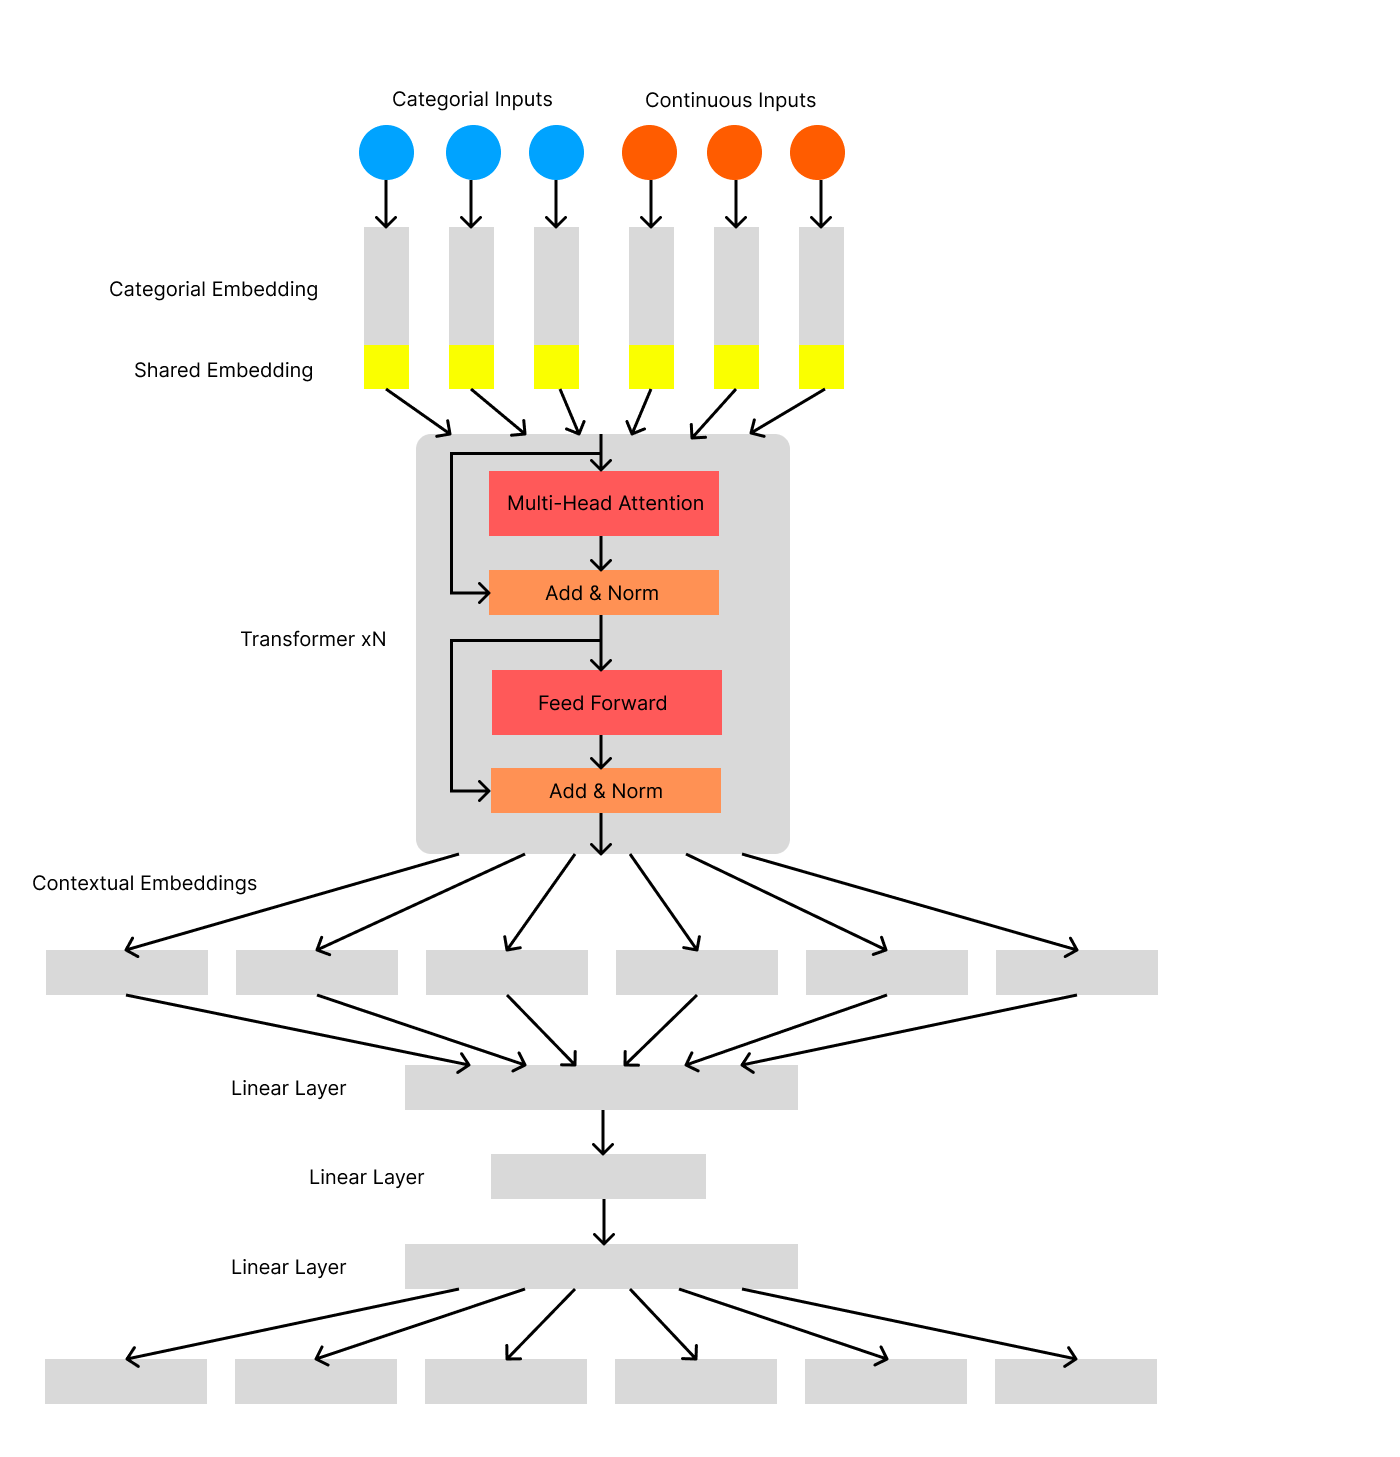
\includegraphics[width=1.2\linewidth]{ft_transformer_autoencoder.png}
	\caption{Architecture of the FT-Transformer autoencoder network.}
	\label{ft_transformer_autoencoder}
\end{figure}

\chapter{Experiments} \label{Experiments}

\section{Comparison of classical Clustering Methods}

\begin{figure}
\begin{center}
\scalebox{0.8}{
	\begin{tabular}{|p{37mm}|p{27mm}|p{27mm}|p{27mm}|p{27mm}|}
	\hline
	&k-means&k-means one-hot&k-prototypes&Gower distance\\\hline
	Abalone&0.1718&\bf{0.1740}&0.1716&0.1614\\ \hline
	Auction Verification&\bf{0.0162}&0.0071&0.0077&0.0062\\ \hline
	Bank Marketing&0.0198&\bf{0.0261}&0.0195&0.0013\\ \hline
	Breast Cancer&\bf{0.7468}&0.7363&0.5925&0.5537\\ \hline
	Census Income&0.1080&\bf{0.1850}&0.1417&0.0043\\ \hline
	Credit Approval&\bf{0.3131}&0.1710&0.1166&0.0035\\ \hline
	Heart Disease&\bf{0.2046}&0.1645&0.1893&0.1408\\ \hline
	Soybean Disease&0.6722&\bf{0.7102}&0.5676&0.6695\\ \hline
	\end{tabular}
}
\end{center}
\caption{Comparison of Normalized Mutual Information of various classical methods on clustering mixed-type datasets.}
\label{classical_comparison_nmi}
\end{figure}

\begin{figure}
\begin{center}
\scalebox{0.8}{
	\begin{tabular}{|p{37mm}|p{27mm}|p{27mm}|p{27mm}|p{27mm}|}
	\hline
	&k-means&k-means one-hot&k-prototypes&Gower distance\\ \hline
	Abalone&0.1353&0.1314&0.1343&\bf{0.1954}\\ \hline
	Auction Verification&0.6647&0.5761&0.5805&\bf{0.8008}\\ \hline
	Bank Marketing&0.7796&0.7866&0.7872&\bf{0.8842}\\ \hline
	Breast Cancer&\bf{0.9605}&0.9502&0.9151&0.9004\\ \hline
	Census Income&0.6082&0.6976&0.6256&\bf{0.7684}\\ \hline
	Credit Approval&\bf{0.8086}&0.7060&0.6662&0.5482\\ \hline
	Heart Disease&0.3344&0.3211&0.4247&\bf{0.5652}\\ \hline
	Soybean Disease&0.5765&\bf{0.5996}&0.4715&0.501\\ \hline
	\end{tabular}
}
\end{center}
\caption{Comparison of Accuracy of various classical methods on clustering mixed-type datasets.}
\label{classical_comparison_acc}
\end{figure}

\begin{figure}
\centering
	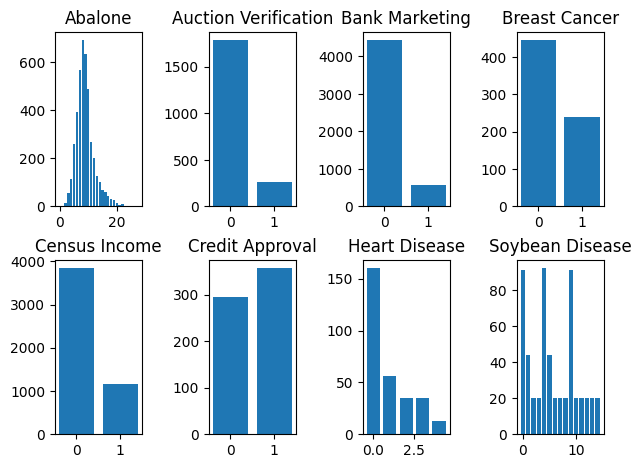
\includegraphics[width=0.8\linewidth]{class-imbalance.png}
	\caption{Number of instances of each target class of each dataset used.}
	\label{class_imbalance}
\end{figure}

Our first comparison is between classical clustering methods for clustering mixed-type data. We evaluated k-means, k-means with one-hot encoding, k-prototypes and gower distance with agglomerative clustering, using average linkage (average distance between each instance of two sets). The results are given by Figure \ref{classical_comparison_nmi} and \ref{classical_comparison_acc}. k-means without any modification for mixed type data shows great Normalized Mutual Information (NMI) scores, k-means with one-hot encoding can improve these on some datasets, but looses on others. k-prototypes can beat k-means only on the Census Income dataset, which does not make it a valid choice for clustering mixed-type data. Gower distance, as explained in Section \ref{Evaluation}, falsely assigns almost all data points to one cluster centroid, which due to the high class imbalance in our datasets as shown in Figure \ref{class_imbalance}, yields high accuracy scores. Therefore more attention should be payed to NMI Scores, on which gower distance does not beat k-means or k-means with one-hot encoding on any dataset. 

\begin{figure}
\begin{center}
\scalebox{0.8}{
	\begin{tabular}{|p{37mm}|p{27mm}|p{27mm}|p{27mm}|p{27mm}|}
	\hline
	&No categorical embedding AE&All features AE&Categorical features AE&All features to categorical features AE\\ \hline
	Abalone&0.1559&0.1695&0.1684&\bf{0.1709}\\ \hline
	Auction Verification&0.0066&0.0012&0.0002&\bf{0.0413}\\ \hline
	Bank Marketing&0.0015&0.0039&\bf{0.0197}&0.0000\\ \hline
	Breast Cancer&\bf{0.7602}&0.7178&0.2878&0.6927\\ \hline
	Census Income&0.0003&0.0241&\bf{0.1024}&0.0042\\ \hline
	Credit Approval&0.0031&\bf{0.0097}&0.0008&0.0028\\ \hline
	Heart Disease&0.1389&0.1663&\bf{0.1848}&0.0947\\ \hline
	Soybean Disease&0.4974&0.4836&0.4169&\bf{0.5426}\\ \hline
	\end{tabular}
}
\end{center}
\caption{Comparison of Normalized Mutual Information of various autoencoder architectures combined with k-means on clustering mixed-type datasets.}
\label{ae_architecture_comparison_nmi}
\end{figure}

\begin{figure}
\begin{center}
\scalebox{0.8}{
	\begin{tabular}{|p{37mm}|p{27mm}|p{27mm}|p{27mm}|p{27mm}|}
	\hline
	&No categorical embedding AE&All features AE&Categorical features AE&All features to categorical features AE\\ \hline
	Abalone&0.1154&\bf{0.1688}&0.1384&0.1348\\ \hline
	Auction Verification&0.5497&0.5893&0.6667&\bf{0.8243}\\ \hline
	Bank Marketing&0.5310&0.7420&\bf{0.7894}&0.7484\\ \hline
	Breast Cancer&\bf{0.9634}&0.9502&0.7013&0.9458\\ \hline
	Census Income&\bf{0.7328}&0.6664&0.5778&0.6216\\ \hline
	Credit Approval&0.5069&0.5176&0.5130&\bf{0.5391}\\ \hline
	Heart Disease&0.3244&0.3278&\bf{0.4013}&0.3545\\ \hline
	Soybean Disease&0.3986&0.4075&0.3292&\bf{0.4413}\\ \hline
	\end{tabular}
}
\end{center}
\caption{Comparison of Accuracy of various autoencoder architectures combined with k-means on clustering mixed-type datasets.}
\label{ae_architecture_comparison_acc}
\end{figure}

The next comparison (Figure \ref{ae_architecture_comparison_nmi} and \ref{ae_architecture_comparison_acc}) revolves around the autoencoder architecture that will be chosen for following modifications. We have the choice between only learning dense representations for categorical features or learning them for all features. Further, we can leave out the categorical embeddings and feed the categorical values as they are into the autoencoder. An autoencoder that gets all features as input in the encoder but only learns to reconstruct the categorical features is also added to the comparison. In order to equalize the autoencoders across all datasets and architectures, the hidden encoded dimension $d_h$ of the autoencoder is calculated by
$$d_h = max(1, min(\left\lfloor d_x/4\right\rceil, \left\lfloor d_y/4\right\rceil)),$$
where $d_x$ is the input dimension of the encoder and $d_y$ the output dimension of the decoder. The number of linear layers $n$ in both the encoder and decoder is given by
$$n = max(1, \left\lfloor log_2 (d_x)\right\rceil).$$
The layer sizes of the encoder are created by always reducing the tensor size by $t_e$ in each linear transformation $h_d - 1$ times, where $t_e$ is calculated as
$$t_e = min(-1, -\left\lfloor \frac{d_x - d_h}{n} \right\rceil).$$
For the decoder, the input dimension $d_x$ in the term is replaced by the output dimension $d_y$:
$$t_d = min(-1, -\left\lfloor \frac{d_y - d_h}{n} \right\rceil).$$
The decoder layer sizes are then calculated by reducing the layer size by $t_d$ from the output layer in each linear transformation $h_d - 1$ times, but inverting the resulting array of layer sizes. This gives us a natural, symmetrical autoencoder structure for each test case (such as Figure \ref{autoencoder_illustration}), which is also used for following experiments. The results do not clearly indicate which autoencoder architecture is the best. Therefore we build upon prior research on mixed-type classification with attention \cite{tab_transformer, ft_transformer}, where a feed-forward network that includes categorical features as well as continuous features is used. This means we choose the autoencoder that includes both categorical and continuous features.

\begin{figure}
\begin{center}
\scalebox{0.8}{
	\begin{tabular}{|p{37mm}|p{27mm}|p{27mm}|p{27mm}|p{27mm}|}
	\hline
	&AE with categorical embeddings&AE with Attention&Transformer N=6&FT-Transformer N=6\\ \hline
	Abalone&0.1603&0.1681&0.1612&\bf{0.1750}\\ \hline
	Auction Verification&\bf{0.1234}&0.0109&0.0045&0.0065\\ \hline
	Bank Marketing&0.0040&\bf{0.0394}&0.0022&0.0040\\ \hline
	Breast Cancer&0.5521&0.1906&\bf{0.5569}&0.4371\\ \hline
	Census Income&\bf{0.1475}&0.0237&0.0056&0.1423\\ \hline
	Credit Approval&0.0123&0.1833&\bf{0.3061}&0.0897\\ \hline
	Heart Disease&0.1550&0.1244&\bf{0.1863}&0.1717\\ \hline
	Soybean Disease&\bf{0.5656}&0.2514&0.3966&0.2755\\ \hline
	\end{tabular}
}
\end{center}
\caption{Comparison of Normalized Mutual Information between an autoencoder with categorical embeddings, an autoencoder using the attention mechanism, a 6-layer Transformer with an autoencoder and a 6-layer FT-Transformer with an autoencoder on clustering mixed-type datasets using k-means.}
\label{attention_comparison_nmi}
\end{figure}

\begin{figure}
\begin{center}
\scalebox{0.8}{
	\begin{tabular}{|p{37mm}|p{27mm}|p{27mm}|p{27mm}|p{27mm}|}
	\hline
	&AE with categorical embeddings&AE with Attention&Transformer N=6&FT-Transformer N=6\\ \hline
	Abalone&0.1503&0.1575&0.1345&\bf{0.1609}\\ \hline
	Auction Verification&\bf{0.8331}&0.6422&0.6393&0.6290\\ \hline
	Bank Marketing&0.7416&0.7044&0.5636&\bf{0.8796}\\ \hline
	Breast Cancer&\bf{0.9136}&0.7277&0.8799&0.8184\\ \hline
	Census Income&0.6740&0.7146&0.6812&\bf{0.7246}\\ \hline
	Credit Approval&0.5360&0.7335&\bf{0.7887}&0.6141\\ \hline
	Heart Disease&0.4448&0.3411&\bf{0.4515}&0.3813\\ \hline
	Soybean Disease&\bf{0.4751}&0.2473&0.3114&0.2420\\ \hline
	\end{tabular}
}
\end{center}
\caption{Comparison of Accuracy between an autoencoder with categorical embeddings, an autoencoder using the attention mechanism, a 6-layer Transformer with an autoencoder and a 6-layer FT-Transformer with an autoencoder on clustering mixed-type datasets using k-means.}
\label{attention_comparison_acc}
\end{figure}

We then compare our proposed architectures, an autoencoder with attention, the Transformer with an autoencoder and the FT-Transformer with an autoencoder. We choose $N = 6$ Transformer layers for both Transformers to utilize the transformer block heavily, but not introduce too much computational complexity. The autoencoder with categorical embeddings uses variable sized embeddings for each categorical feature (that are being concatenated lengthwise), where the embedding dimension is calculated based on the number of classes in that feature, as explained in Section \ref{Column Embeddings}. The attention autoencoder as well as both Transformer autoencoders use fixed size embeddings of size 32, which allows the embeddings to be stacked on top of each other, as explained in Section \ref{Attention}. The results (Figure \ref{attention_comparison_nmi} and \ref{attention_comparison_acc}) show that the attention can benefit clustering on some datasets, but leads to a loss in performance on other datasets.

\begin{figure}
\begin{center}
\scalebox{0.8}{
	\begin{tabular}{|p{37mm}|p{10mm}|p{24mm}|p{24mm}|p{24mm}|p{24mm}|}
	\hline
	&&AE with categorical embeddings&Attention&Transformer N=6&FT-Transformer N=6\\ \hline
	&DEC&0.1585&0.1630&0.1642&0.1520\\
	Abalone&IDEC&0.1501&0.1623&0.1653&0.1660\\
	&DCN&0.1574&\bf{0.1717}&0.1671&0.1704\\ \hline

	&DEC&0.0179&0.0203&0.0446&0.0000\\
	Auction Verification&IDEC&0.0179&0.0203&0.0444&0.0000\\
	&DCN&0.0179&0.0203&\bf{0.0484}&0.0000\\ \hline

	&DEC&\bf{0.0195}&0.0023&0.0000&0.0015\\
	Bank Marketing&IDEC&0.0172&0.0023&0.0000&0.0012\\
	&DCN&\bf{0.0195}&0.0023&0.0000&0.0006\\ \hline

	&DEC&0.7284&0.2185&0.5991&0.2062\\
	Breast Cancer&IDEC&0.7284&0.2185&0.2244&0.2062\\
	&DCN&\bf{0.7333}&0.2185&0.2062&0.2062\\ \hline

	&DEC&\bf{0.0915}&0.0663&0.0689&0.1333\\
	Census Income&IDEC&0.0911&0.0663&0.0689&0.1333\\
	&DCN&\bf{0.0915}&0.0663&0.0689&0.1333\\ \hline

	&DEC&0.0027&0.0000&0.0036&\bf{0.0725}\\
	Credit Approval	&IDEC&0.0024&0.0000&0.0036&\bf{0.0725}\\
	&DCN&0.0024&0.0000&0.0036&\bf{0.0725}\\ \hline

	&DEC&0.1273&0.1599&0.1494&0.2434\\
	Heart Disease&IDEC&0.1273&0.1599&0.1503&0.2434\\
	&DCN&0.1268&0.1599&0.1558&\bf{0.2473}\\ \hline

	&DEC&0.3878&0.5168&0.2605&0.2605\\
	Soybean Disease&IDEC&0.3866&\bf{0.6532}&0.2684&0.2684\\
	&DCN&0.3930&0.6306&0.2605&0.2605\\ \hline
	\end{tabular}
}
\end{center}
\caption{Comparison of Normalized Mutual Information between an autoencoder with categorical embeddings, an autoencoder with attention, a 6-layer Transformer with an autoencoder and a 6-layer FT-Transformer with an autoencoder on clustering mixed-type datasets. DEC, IDEC and DCN were used as clustering methods.}
\label{deep_comparison_nmi}
\end{figure}

\begin{figure}
\begin{center}
\scalebox{0.8}{
	\begin{tabular}{|p{37mm}|p{10mm}|p{24mm}|p{24mm}|p{24mm}|p{24mm}|}
	\hline
	&&AE with categorical embeddings&Attention&Transformer N=6&FT-Transformer N=6\\ \hline
	&DEC&0.1621&0.1286&0.1549&0.1858\\
	Abalone&IDEC&0.1472&0.1384&0.1559&0.1678\\
	&DCN&0.1676&0.1585&0.1685&\bf{0.2107}\\ \hline

	&DEC&0.6676&0.6760&0.6848&\bf{0.7445}\\
	Auction Verification&IDEC&0.6676&0.6760&0.6843&\bf{0.7445}\\
	&DCN&0.6676&0.6760&0.6569&\bf{0.7445}\\ \hline

	&DEC&0.5712&0.7010&0.7602&0.7936\\
	Bank Marketing&IDEC&0.6162&0.7010&0.7602&0.7950\\
	&DCN&0.5712&0.7010&0.7602&\bf{0.8172}\\ \hline

	&DEC&0.9458&0.7467&0.8990&0.7350\\
	Breast Cancer&IDEC&0.9458&0.7467&0.7745&0.7350\\
	&DCN&\bf{0.9473}&0.7467&0.7350&0.7350\\ \hline

	&DEC&0.6488&\bf{0.7414}&0.6284&0.7236\\
	Census Income&IDEC&0.6486&\bf{0.7414}&0.6284&0.7236\\
	&DCN&0.6488&\bf{0.7414}&0.6284&0.7236\\ \hline

	&DEC&0.5375&0.5299&0.5467&\bf{0.5697}\\
	Credit Approval&IDEC&0.5360&0.5299&0.5467&\bf{0.5697}\\
	&DCN&0.5360&0.5299&0.5467&\bf{0.5697}\\ \hline

	&DEC&0.2977&0.3445&0.3378&\bf{0.5652}\\
	Heart Disease&IDEC&0.2977&0.3445&0.3344&\bf{0.5652}\\
	&DCN&0.3010&0.3445&0.3445&0.5585\\ \hline

	&DEC&0.2544&0.4431&0.2278&0.2278\\
	Soybean Disease&IDEC&0.2544&\bf{0.5552}&0.2295&0.2295\\
	&DCN&0.2669&0.5125&0.2278&0.2278\\ \hline
	\end{tabular}
}
\end{center}
\caption{Comparison of Accuracy between an autoencoder with categorical embeddings, an autoencoder with attention, a 6-layer Transformer with an autoencoder and a 6-layer FT-Transformer with an autoencoder on clustering mixed-type datasets. DEC, IDEC and DCN were used as clustering methods.}
\label{deep_comparison_acc}
\end{figure}

At last, we use the models from the previous comparison, but use the deep clustering techniques DEC, IDEC and DCN (Section \ref{Deep Clustering}). The Normalized Mutual Information results of these methods (Figure \ref{deep_comparison_nmi}) do not indicate that deep clustering methods are particular useful for clustering mixed-type data.

\begin{figure}
\begin{center}
\scalebox{0.8}{
	\begin{tabular}{|p{37mm}|p{36mm}|p{36mm}|p{36mm}|}
	\hline
	&1st&2nd&3rd\\ \hline
	Abalone&\cellcolor{yellow}FT-Transformer (0.1750)&\cellcolor{green}k-means one-hot (0.1740)&\cellcolor{green}k-means (0.1718)\\ \hline
	Auction Verification&\cellcolor{cyan}AE with Column Embeddings (0.1234)&\cellcolor{magenta}DCN Transformer (0.0484)&\cellcolor{magenta}DEC Transformer(0.0446)\\ \hline
	Bank Marketing&\cellcolor{yellow}AE with Attention (0.0394)&\cellcolor{green}k-means one-hot (0.0261)&\cellcolor{green}k-means (0.0198)\\ \hline
	Breast Cancer&\cellcolor{cyan}Basic AE (0.7602)&\cellcolor{green}k-means (0.7468)&\cellcolor{green}k-means one-hot (0.7363)\\ \hline
	Census Income&\cellcolor{green}k-means one-hot (0.1850)&\cellcolor{cyan}AE with Column Embeddings (0.1475)&\cellcolor{yellow}FT-Transformer (0.1423)\\ \hline
	Credit Approval&\cellcolor{green}k-means (0.3131)&\cellcolor{yellow}Transformer (0.3061)&\cellcolor{yellow}AE with Attention (0.1833)\\ \hline
	Heart Disease&\cellcolor{magenta}DCN FT-Transformer (0.2473)&\cellcolor{magenta}DEC/IDEC FT-Transformer (0.2434)&\cellcolor{green}k-means (0.2046)\\ \hline
	Soybean Disease&\cellcolor{green}k-means one-hot (0.7102)&\cellcolor{green}k-means (0.6722)&\cellcolor{green}Gower distance (0.6695)\\ \hline
	\end{tabular}
}
\end{center}
\caption{Best Normalized Mutual Information results (in parenthesis) across all clustering methods. Classical methods are colored in green, methods using an autoencoder with k-means are colored cyan, methods using an autoencoder and attention or a transformer mechanism are colored yellow and methods using DEC, IDEC or DCN are colored magenta.}
\label{final_comparison_nmi}
\end{figure}
	
\chapter{Conclusion}
